\posterbox[adjusted title=Testing \& Results]
  {name=algorithm,column=4,between=title and references}{
  \vspace{1cm}
  {\small The software~\cite{dortogul} is tested on various graph sizes/densities:}
  
  \vspace{1cm}
  {\Large \textbf{Key Findings}}
  
  \begin{itemize}
      \item The software can partition graphs of any density when the graph's size is less than 50.
      \item When the graph's size is greater than 50, complexity of the problem increases very quickly and the software can only partition sparse graphs.
      \item On average, weightless version of the problem takes slightly more time to solve than the weighted version.

  \end{itemize}

  \begin{minipage}{.5\linewidth}
        \centering
        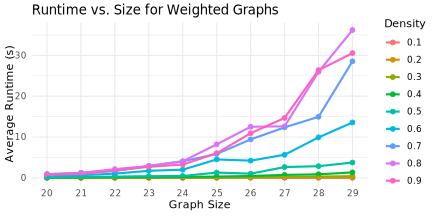
\includegraphics[width=\linewidth]{images/p1}\\
        {\footnotesize (a)}
    \end{minipage}%
    \begin{minipage}{0.5\linewidth}
        \centering
        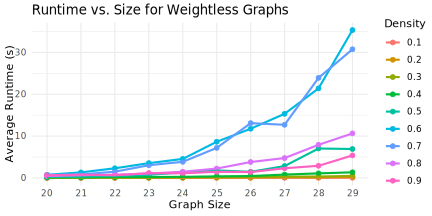
\includegraphics[width=\linewidth]{images/p2}
        {\footnotesize (b)}
    \end{minipage}
    \begin{center}
        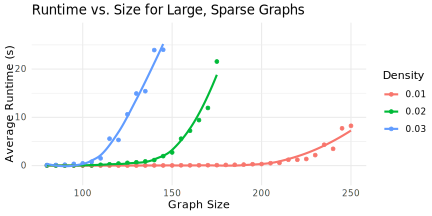
\includegraphics[width=\linewidth]{images/p3}
        {\footnotesize (c)}

        {\small Figure 4: Plots of the runtime of the algorithm}
    \end{center}
    
\vspace{1cm}
{\Large \textbf{Showcase}}

\begin{minipage}{.5\linewidth}
        \centering
        \includesvg[width=\linewidth]{images/graph20}
    \end{minipage}%
    \begin{minipage}{0.5\linewidth}
        \centering
        \includesvg[width=\linewidth]{images/graph60}
    \end{minipage}

    \begin{minipage}{.5\linewidth}
        \centering
        \includesvg[width=\linewidth]{images/wgraph20}
    \end{minipage}%
    \begin{minipage}{0.5\linewidth}
        \centering
        \includesvg[width=\linewidth]{images/wgraph60}
    \end{minipage}
    
  
}